\begin{enumerate}[label=\thesubsection.\arabic*, ref=\thesubsection.\theenumi]
\item 
If the angle between two tangents drawn from an external point P to a circle of radius $a$ and centre O, is $60^{\circ}$, then find the length of OP.
\hfill (CBSE~2017)
\\
\solution
Let $\vec{T}_1$ and $\vec{T}_2$ be the points of contact of the tangents from $\vec{P}$. From \eqref{eq:EE26BTECH11229-tangent-equal},
\begin{align}
	\norm{\vec{P}-\vec{T}_1} = \norm{\vec{P}-\vec{T}_2}
\end{align}
Also $\norm{\vec{O}-\vec{T}_1} = \norm{\vec{O}-\vec{T}_2} = a$ and $\vec{O}\vec{P}$ is common. So the triangles $\vec{O}\vec{T}_1\vec{P}$ and $\vec{O}\vec{T}_2\vec{P}$ are congruent, and $\vec{O}\vec{P}$ bisects the angle between the tangents,
\begin{align}
	\angle \vec{O}\vec{P}\vec{T}_1 = \frac{60^{\circ}}{2} = 30^{\circ}
\end{align}
From \eqref{eq:EE26BTECH11229-tangent-perp}, the triangle $\vec{O}\vec{T}_1\vec{P}$ is right angled at $\vec{T}_1$. Using \eqref{eq:EE26BTECH11229-trig},
\begin{align}
	\sin 30^{\circ} &= \frac{a}{\norm{\vec{O}-\vec{P}}}
	\\
	\implies \norm{\vec{O}-\vec{P}} &= \frac{a}{\frac{1}{2}} = 2a
\end{align}
\item 
A circle touches all the four sides of a quadrilateral ABCD. Prove that 
\begin{align*}
	AB + CD = BC + DA
\end{align*}
\hfill (CBSE~2017)
\\
\solution
Let the circle touch $AB$, $BC$, $CD$ and $DA$ at $\vec{P}$, $\vec{Q}$, $\vec{R}$ and $\vec{S}$ respectively. The tangents drawn from each of $\vec{A}$, $\vec{B}$, $\vec{C}$ and $\vec{D}$ are equal, from \eqref{eq:EE26BTECH11229-tangent-equal}. Hence,
\begin{align}
	AP = AS, \quad BP = BQ, \quad CR = CQ, \quad DR = DS
	\label{eq:EE26BTECH11229-Prob_5-1}
\end{align}
Adding the above,
\begin{align}
	\brak{AP + BP} + \brak{CR + DR} = \brak{AS + DS} + \brak{BQ + CQ}
\end{align}
Since $\vec{P}$ lies on $AB$, $\vec{R}$ on $CD$, $\vec{S}$ on $DA$ and $\vec{Q}$ on $BC$, 
\begin{align}
	AP + BP = AB, \quad CR + DR = CD, \quad AS + DS = DA, \quad BQ + CQ = BC
\end{align}
Substituting in the above,
\begin{align}
	AB + CD = BC + DA
\end{align}
\item 
If the distances of $\vec{P}\brak{x, y}$ from $\vec{A}\brak{5, 1}$ and $\vec{B}\brak{-1, 5}$ are equal, then prove that $3x = 2y$.
\hfill (CBSE~2017)
\\
\solution
Let
\begin{align}
	\vec{x} = \myvec{x \\ y}, \quad \vec{A} = \myvec{5 \\ 1}, \quad \vec{B} = \myvec{-1 \\ 5}
\end{align}
Then
\begin{align}
	\vec{A} - \vec{B} = \myvec{6 \\ -4}, \quad
	\norm{\vec{A}}^2 = 26, \quad \norm{\vec{B}}^2 = 26
\end{align}
Substituting in \eqref{eq:EE26BTECH11229-perp-bisector},
\begin{align}
	\myvec{6 & -4}\myvec{x \\ y} &= \frac{26 - 26}{2} = 0
	\\
	\implies 6x - 4y &= 0
	\\
	\therefore 3x &= 2y
\end{align}
\item 
Find the value of $p$, for which one root of the quadratic equation $px^2 - 14x + 8 = 0$ is 6 times the other.
\hfill (CBSE~2017)
\\
\solution
Let the roots be $\alpha$ and $6\alpha$. From \eqref{eq:EE26BTECH11229-quad-roots},
\begin{align}
	\alpha + 6\alpha &= \frac{14}{p}
	\label{eq:EE26BTECH11229-Prob_9-1}
	\\
	\alpha \brak{6\alpha} &= \frac{8}{p}
	\label{eq:EE26BTECH11229-Prob_9-2}
\end{align}
From \eqref{eq:EE26BTECH11229-Prob_9-1}, 
\begin{align}
	\alpha = \frac{2}{p}
\end{align}
Substituting in \eqref{eq:EE26BTECH11229-Prob_9-2},
\begin{align}
	\frac{24}{p^2} &= \frac{8}{p}
	\\
	\implies p &= 3
\end{align}
For $p=3$, the roots are $4$ and $\frac{2}{3}$, and indeed $4 = 6\brak{\frac{2}{3}}$.
The following code verifies the solution
\begin{lstlisting}[frame=single, basicstyle=\rmfamily, escapeinside={(*@}{@*)}]
(*@\makebox[\dimexpr\linewidth-2\fboxsep-2\fboxrule\relax][c]{codes/quadratic.c}@*)
\end{lstlisting}
\item 
For what value of $n$, are the $n^{\text{th}}$ terms of two A.Ps $63, 65, 67, \ldots$ and $3, 10, 17, \ldots$ equal ?
\hfill (CBSE~2017)
\\
\solution
For the first A.P., $a = 63$, $d = 2$ and for the second A.P., $a = 3$, $d = 7$. Equating the $n^{\text{th}}$ terms using \eqref{eq:EE26BTECH11229-ap-nth},
\begin{align}
	63 + \brak{n-1}2 &= 3 + \brak{n-1}7
	\\
	\implies 5\brak{n-1} &= 60
	\\
	\therefore n &= 13
\end{align}
Both terms are then equal to $87$.
The following code verifies the solution
\begin{lstlisting}[frame=single, basicstyle=\rmfamily, escapeinside={(*@}{@*)}]
(*@\makebox[\dimexpr\linewidth-2\fboxsep-2\fboxrule\relax][c]{codes/ap\_equal.c}@*)
\end{lstlisting}
\item 
On a straight line passing through the foot of a tower, two points C and D are at distances of 4 m and 16 m from the foot respectively. If the angles of elevation from C and D of the top of the tower are complementary, then find the height of the tower.
\hfill (CBSE~2017)
\\
\solution
Let $h$ be the height of the tower and $\theta$ be the angle of elevation from $\vec{C}$. The angle of elevation from $\vec{D}$ is then $90^{\circ} - \theta$. From \eqref{eq:EE26BTECH11229-trig},
\begin{align}
	\tan\theta = \frac{h}{4}, \quad \tan\brak{90^{\circ}-\theta} = \frac{h}{16}
\end{align}
From \eqref{eq:EE26BTECH11229-tan-comp},
\begin{align}
	\frac{h}{4}\cdot\frac{h}{16} &= 1
	\\
	\implies h^2 &= 64
	\\
	\therefore h &= 8 \text{ m}
\end{align}
The following code generates \figref{fig:EE26BTECH11229-5}
\begin{lstlisting}[frame=single, basicstyle=\rmfamily, escapeinside={(*@}{@*)}]
(*@\makebox[\dimexpr\linewidth-2\fboxsep-2\fboxrule\relax][c]{codes/trig\_height.py}@*)
\end{lstlisting}
\begin{figure}[H]
    \centering
    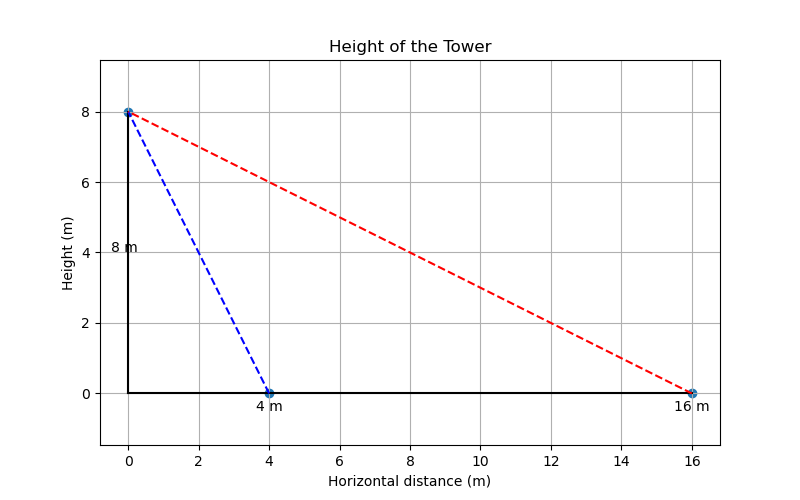
\includegraphics[width=0.75\linewidth]{figs/trig_height.png}
    \caption{Tower and the angles of elevation}
    \label{fig:EE26BTECH11229-5}
\end{figure}
\item 
Three semicircles each of diameter 3 cm, a circle of diameter 4.5 cm and a semicircle of radius 4.5 cm are drawn in the given figure. Find the area of the shaded region.
\hfill (CBSE~2017)
\begin{figure}[H]
	\centering
\begin{tikzpicture}[scale=0.8]
% large semicircle (shaded)
\fill[pattern=north east lines] (-4.5,0) arc (180:0:4.5) -- cycle;
% unshaded: circle and the two upper small semicircles
\fill[white] (0,2.25) circle (2.25);
\fill[white] (-4.5,0) arc (180:0:1.5) -- cycle;
\fill[white] (1.5,0) arc (180:0:1.5) -- cycle;
% lower small semicircle (shaded)
\fill[pattern=north east lines] (-1.5,0) arc (180:360:1.5) -- cycle;

% outlines
\draw (-4.5,0) arc (180:0:4.5) -- cycle;
\draw (0,2.25) circle (2.25);
\draw (-4.5,0) arc (180:0:1.5);
\draw (1.5,0) arc (180:0:1.5);
\draw (-1.5,0) arc (180:360:1.5);

% dimensions
\draw[dotted] (-4.5,0) -- (-4.5,-2.2);
\draw[dotted] (-1.5,0) -- (-1.5,-2.2);
\draw[dotted] (1.5,0) -- (1.5,-2.2);
\draw[dotted] (4.5,0) -- (4.5,-2.2);
\draw[<->] (-4.5,-2) -- (-1.5,-2) node[midway,below] {3 cm};
\draw[<->] (-1.5,-2) -- (1.5,-2) node[midway,below] {3 cm};
\draw[<->] (1.5,-2) -- (4.5,-2) node[midway,below] {3 cm};
\end{tikzpicture}
\caption{}
    \label{fig:EE26BTECH11229-1}
\end{figure}
\solution
In \figref{fig:EE26BTECH11229-1}, the radii are
\begin{align}
	R = \frac{9}{2} \text{ cm (large semicircle)}, \quad
	r = \frac{3}{2} \text{ cm (small semicircles)}, \quad
	\rho = \frac{9}{4} \text{ cm (circle)}
\end{align}
The shaded region is the large semicircle, excluding the circle and the two upper small semicircles, and including the lower small semicircle. Using \eqref{eq:EE26BTECH11229-area-circle}, the area is
\begin{align}
	A &= \frac{1}{2}\pi R^2 - \pi\rho^2 - 2\brak{\frac{1}{2}\pi r^2} + \frac{1}{2}\pi r^2
	\\
	&= \frac{1}{2}\pi R^2 - \pi\rho^2 - \frac{1}{2}\pi r^2
	\\
	&= \pi\brak{\frac{81}{8} - \frac{81}{16} - \frac{9}{8}}
	= \frac{63\pi}{16}
\end{align}
Substituting $\pi = \frac{22}{7}$,
\begin{align}
	A = \frac{63}{16}\times\frac{22}{7} = \frac{99}{8} = 12.375 \text{ cm}^2
\end{align}
The following code generates \figref{fig:EE26BTECH11229-9}
\begin{lstlisting}[frame=single, basicstyle=\rmfamily, escapeinside={(*@}{@*)}]
(*@\makebox[\dimexpr\linewidth-2\fboxsep-2\fboxrule\relax][c]{codes/shaded\_area.py}@*)
\end{lstlisting}
\begin{figure}[H]
    \centering
    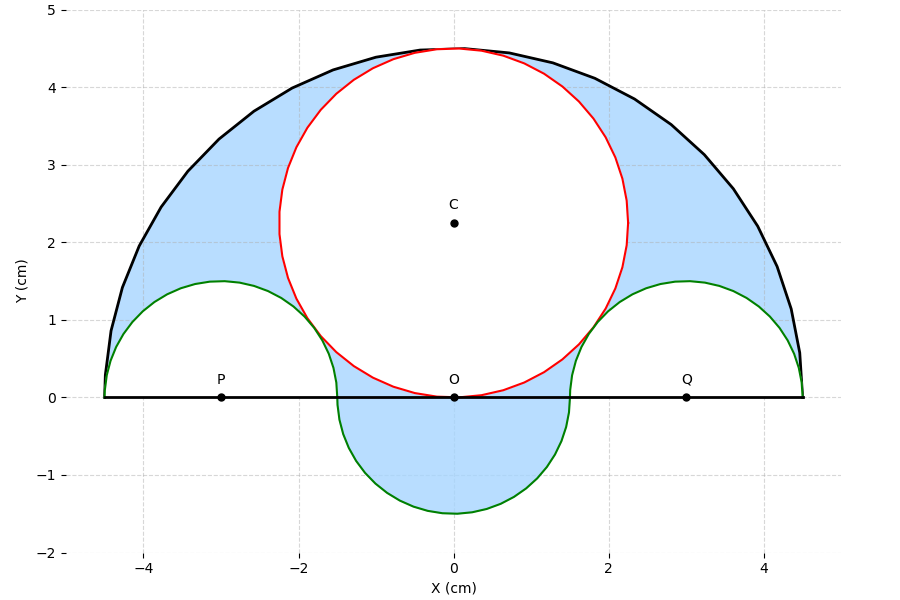
\includegraphics[width=0.75\linewidth]{figs/shaded_region.png}
    \caption{Shaded region}
    \label{fig:EE26BTECH11229-9}
\end{figure}
\item 
In what ratio does the point $\brak{\frac{24}{11}, y}$ divide the line segment joining the points $\vec{P}\brak{2, -2}$ and $\vec{Q}\brak{3, 7}$ ? Also find the value of $y$.
\hfill (CBSE~2017)
\\
\solution
Let the ratio be $k:1$. From \eqref{eq:EE26BTECH11229-section},
\begin{align}
	\myvec{\frac{24}{11} \\ y} = \frac{k\myvec{3 \\ 7} + \myvec{2 \\ -2}}{k+1}
\end{align}
Considering the first row,
\begin{align}
	\frac{24}{11} &= \frac{3k+2}{k+1}
	\\
	\implies 24k + 24 &= 33k + 22
	\\
	\implies k &= \frac{2}{9}
\end{align}
Thus, the ratio is $2:9$. Considering the second row,
\begin{align}
	y = \frac{7k - 2}{k+1} = \frac{\frac{14}{9} - 2}{\frac{11}{9}} = -\frac{4}{11}
\end{align}
The following code verifies the solution
\begin{lstlisting}[frame=single, basicstyle=\rmfamily, escapeinside={(*@}{@*)}]
(*@\makebox[\dimexpr\linewidth-2\fboxsep-2\fboxrule\relax][c]{codes/section.c}@*)
\end{lstlisting}
\item 
Water in a canal, 5.4 m wide and 1.8 m deep, is flowing with a speed of 25 km/hour. How much area can it irrigate in 40 minutes, if 10 cm of standing water is required for irrigation ?
\hfill (CBSE~2017)
\\
\solution
The cross-sectional area, speed and time are
\begin{align}
	A = 5.4 \times 1.8 \text{ m}^2, \quad v = 25000 \text{ m/h}, \quad t = \frac{40}{60} = \frac{2}{3} \text{ h}
\end{align}
From \eqref{eq:EE26BTECH11229-flow}, the volume of water that flows in 40 minutes is
\begin{align}
	V = 5.4 \times 1.8 \times 25000 \times \frac{2}{3} = 162000 \text{ m}^3
\end{align}
If this water stands at a depth of $10 \text{ cm} = 0.1 \text{ m}$ over an area $S$,
\begin{align}
	S \times 0.1 &= 162000
	\\
	\implies S &= 1620000 \text{ m}^2 = 162 \text{ hectares}
\end{align}
\item 
In the given figure, two concentric circles with centre O have radii 21 cm and 42 cm. If $\angle AOB = 60^{\circ}$, find the area of the shaded region.
\hfill [Use $\pi = \frac{22}{7}$] \hfill (CBSE~2017)
\begin{figure}[H]
	\centering
\begin{tikzpicture}[scale=1.6]
\coordinate (O) at (0,0);
\coordinate (A) at (240:2);
\coordinate (B) at (300:2);
\coordinate (C) at (240:1);
\coordinate (D) at (300:1);
% shaded ring
\fill[pattern=vertical lines, even odd rule] (O) circle (2) circle (1);
% unshaded part of the ring inside the 60 degree angle
\fill[white] (C) -- (A) arc (240:300:2) -- (D) arc (300:240:1) -- cycle;
% outlines
\draw (O) circle (2);
\draw (O) circle (1);
\draw (O) -- (A);
\draw (O) -- (B);
\draw (A) arc (240:300:2);
\draw (0.0,-0.45) node {$60^{\circ}$};
\fill (O) circle (0.025) node[above] {O};
\node[below left] at (A) {A};
\node[below right] at (B) {B};
\node[left] at (C) {C};
\node[right] at (D) {D};
\end{tikzpicture}
\caption{}
    \label{fig:EE26BTECH11229-2}
\end{figure}
\solution
In \figref{fig:EE26BTECH11229-2}, the radii are $R = 42$ cm and $r = 21$ cm. The shaded region is the ring between the circles, excluding the part of the ring inside the $60^{\circ}$ angle. From \eqref{eq:EE26BTECH11229-sector},
\begin{align}
	A &= \pi\brak{R^2 - r^2} - \frac{60^{\circ}}{360^{\circ}}\pi\brak{R^2 - r^2}
	\\
	&= \frac{5}{6}\pi\brak{42^2 - 21^2}
	= \frac{5}{6}\times\frac{22}{7}\times 1323
\end{align}
yielding
\begin{align}
	A = 3465 \text{ cm}^2
\end{align}
The following code generates \figref{fig:EE26BTECH11229-6}
\begin{lstlisting}[frame=single, basicstyle=\rmfamily, escapeinside={(*@}{@*)}]
(*@\makebox[\dimexpr\linewidth-2\fboxsep-2\fboxrule\relax][c]{codes/sector\_area.py}@*)
\end{lstlisting}
\begin{figure}[H]
    \centering
    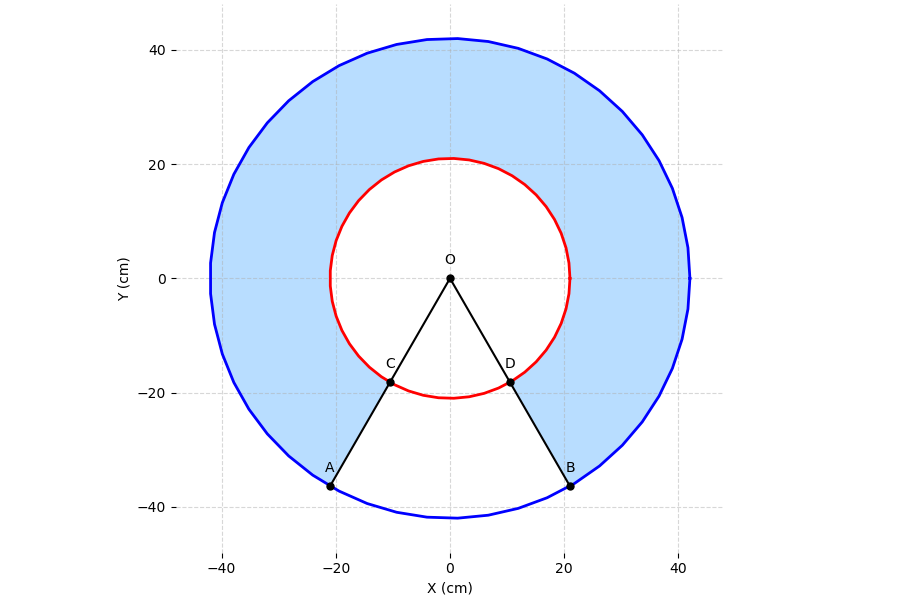
\includegraphics[width=0.75\linewidth]{figs/sector_area.png}
    \caption{Annular sector}
    \label{fig:EE26BTECH11229-6}
\end{figure}
\item 
The dimensions of a solid iron cuboid are $4.4 \text{ m} \times 2.6 \text{ m} \times 1.0 \text{ m}$. It is melted and recast into a hollow cylindrical pipe of 30 cm inner radius and thickness 5 cm. Find the length of the pipe.
\hfill (CBSE~2017)
\\
\solution
The volume of the cuboid is
\begin{align}
	V = 4.4 \times 2.6 \times 1.0 = 11.44 \text{ m}^3
\end{align}
The inner and outer radii of the pipe are $r = 0.3$ m and $R = 0.3 + 0.05 = 0.35$ m. Let $h$ be the length of the pipe. Equating the volumes using \eqref{eq:EE26BTECH11229-hollow-cyl},
\begin{align}
	\frac{22}{7}\brak{0.35^2 - 0.3^2}h &= 11.44
	\\
	\implies \frac{22}{7}\times 0.0325\, h &= 11.44
	\\
	\therefore h &= 112 \text{ m}
\end{align}
The following code verifies the solution
\begin{lstlisting}[frame=single, basicstyle=\rmfamily, escapeinside={(*@}{@*)}]
(*@\makebox[\dimexpr\linewidth-2\fboxsep-2\fboxrule\relax][c]{codes/cylinder.c}@*)
\end{lstlisting}
\item 
A toy is in the form of a cone of radius 3.5 cm mounted on a hemisphere of same radius on its circular face. The total height of the toy is 15.5 cm. Find the total surface area of the toy.
\hfill (CBSE~2017)
\\
\solution
The radius is $r = 3.5$ cm. The height of the cone is
\begin{align}
	h = 15.5 - 3.5 = 12 \text{ cm}
\end{align}
From \eqref{eq:EE26BTECH11229-cone}, the slant height is
\begin{align}
	l = \sqrt{12^2 + 3.5^2} = \sqrt{156.25} = 12.5 \text{ cm}
\end{align}
The total surface area is the sum of the curved surface areas of the cone and the hemisphere, from \eqref{eq:EE26BTECH11229-cone} and \eqref{eq:EE26BTECH11229-hemisphere},
\begin{align}
	A &= \pi r l + 2\pi r^2 = \pi r\brak{l + 2r}
	\\
	&= \frac{22}{7}\times 3.5 \times \brak{12.5 + 7}
	= 214.5 \text{ cm}^2
\end{align}
The following code generates \figref{fig:EE26BTECH11229-7}
\begin{lstlisting}[frame=single, basicstyle=\rmfamily, escapeinside={(*@}{@*)}]
(*@\makebox[\dimexpr\linewidth-2\fboxsep-2\fboxrule\relax][c]{codes/cone\_hemisphere.py}@*)
\end{lstlisting}
\begin{figure}[H]
    \centering
    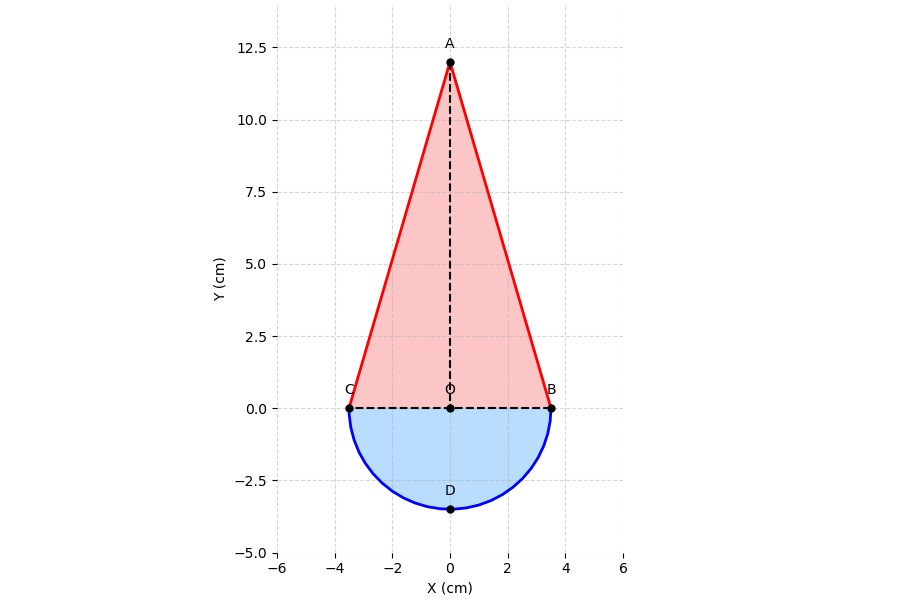
\includegraphics[width=0.75\linewidth]{figs/cone_hemisphere.png}
    \caption{Cone mounted on a hemisphere}
    \label{fig:EE26BTECH11229-7}
\end{figure}
\item 
How many terms of an A.P. $9, 17, 25, \ldots$ must be taken to give a sum of 636 ?
\hfill (CBSE~2017)
\\
\solution
Here $a = 9$ and $d = 8$. From \eqref{eq:EE26BTECH11229-ap-sum},
\begin{align}
	\frac{n}{2}\sbrak{18 + 8\brak{n-1}} &= 636
	\\
	\implies 4n^2 + 5n - 636 &= 0
\end{align}
From \eqref{eq:EE26BTECH11229-quad-formula},
\begin{align}
	n = \frac{-5 \pm \sqrt{25 + 10176}}{8} = \frac{-5 \pm 101}{8}
\end{align}
Since $n$ is positive,
\begin{align}
	n = 12
\end{align}
The following code verifies the solution
\begin{lstlisting}[frame=single, basicstyle=\rmfamily, escapeinside={(*@}{@*)}]
(*@\makebox[\dimexpr\linewidth-2\fboxsep-2\fboxrule\relax][c]{codes/ap\_sum.c}@*)
\end{lstlisting}
\item 
If the roots of the equation $\brak{a^2 + b^2}x^2 - 2\brak{ac + bd}x + \brak{c^2 + d^2} = 0$ are equal, prove that $\frac{a}{b} = \frac{c}{d}$.
\hfill (CBSE~2017)
\\
\solution
From \eqref{eq:EE26BTECH11229-quad-equal},
\begin{align}
	4\brak{ac + bd}^2 - 4\brak{a^2 + b^2}\brak{c^2 + d^2} &= 0
	\\
	\implies a^2c^2 + 2abcd + b^2d^2 &= a^2c^2 + a^2d^2 + b^2c^2 + b^2d^2
	\\
	\implies a^2d^2 - 2abcd + b^2c^2 &= 0
	\\
	\implies \brak{ad - bc}^2 &= 0
	\\
	\implies ad &= bc
\end{align}
Dividing by $bd$,
\begin{align}
	\frac{a}{b} = \frac{c}{d}
\end{align}
\item 
If the points $\vec{A}\brak{k+1, 2k}$, $\vec{B}\brak{3k, 2k+3}$ and $\vec{C}\brak{5k-1, 5k}$ are collinear, then find the value of $k$.
\hfill (CBSE~2017)
\\
\solution
Let
\begin{align}
	\vec{B} - \vec{A} = \myvec{2k-1 \\ 3}, \quad \vec{C} - \vec{A} = \myvec{4k-2 \\ 3k}
\end{align}
From \eqref{eq:EE26BTECH11229-collinear}, the points are collinear if
\begin{align}
	\mydet{\myvec{2k-1 & 4k-2 \\ 3 & 3k}} &= 0
	\\
	\implies 3k\brak{2k-1} - 3\brak{4k-2} &= 0
	\\
	\implies 2k^2 - 5k + 2 &= 0
	\\
	\implies \brak{2k-1}\brak{k-2} &= 0
\end{align}
Hence,
\begin{align}
	k = \frac{1}{2} \quad \text{or} \quad k = 2
\end{align}
\item 
Two different dice are thrown together. Find the probability that the numbers obtained have
\begin{enumerate}
	\item even sum, and
	\item even product.
\end{enumerate}
\hfill (CBSE~2017)
\\
\solution
The total number of equally likely outcomes is $N = 36$.
\begin{enumerate}
\item The sum is even if both numbers are even or both are odd. There are $3 \times 3 = 9$ outcomes of each type. From \eqref{eq:EE26BTECH11229-prob-def},
\begin{align}
	\pr{\text{even sum}} = \frac{9 + 9}{36} = \frac{1}{2}
\end{align}
\item The product is odd only if both numbers are odd, which gives $3 \times 3 = 9$ outcomes. Thus,
\begin{align}
	\pr{\text{odd product}} = \frac{9}{36} = \frac{1}{4}
\end{align}
Using the complement in \eqref{eq:EE26BTECH11229-prob-def},
\begin{align}
	\pr{\text{even product}} = 1 - \frac{1}{4} = \frac{3}{4}
\end{align}
\end{enumerate}
The following code verifies the solution
\begin{lstlisting}[frame=single, basicstyle=\rmfamily, escapeinside={(*@}{@*)}]
(*@\makebox[\dimexpr\linewidth-2\fboxsep-2\fboxrule\relax][c]{codes/dice\_prob.c}@*)
\end{lstlisting}
\item 
In the given figure, $XY$ and $X^{\prime}Y^{\prime}$ are two parallel tangents to a circle with centre O and another tangent $AB$ with point of contact $C$, is intersecting $XY$ at $A$ and $X^{\prime}Y^{\prime}$ at $B$. Prove that $\angle AOB = 90^{\circ}$.
\hfill (CBSE~2017)
\begin{figure}[H]
	\centering
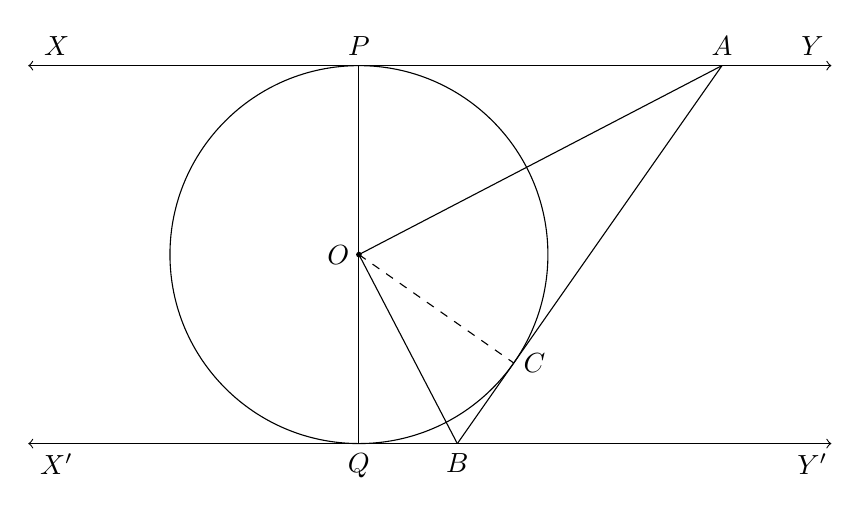
\begin{tikzpicture}[scale=1.2]
\coordinate (O) at (0,0);
\coordinate (P) at (0,2);
\coordinate (Q) at (0,-2);
\coordinate (C) at (-35:2);
\coordinate (A) at ({(2-2*sin(-35))/cos(-35)},2);
\coordinate (B) at ({(2+2*sin(-35))/cos(-35)},-2);
% circle and parallel tangents
\draw (O) circle (2);
\draw[<->] (-3.5,2) -- (5,2);
\draw[<->] (-3.5,-2) -- (5,-2);
% diameter PQ and tangent AB
\draw (P) -- (Q);
\draw (A) -- (B);
\draw (O) -- (A);
\draw (O) -- (B);
\draw[dashed] (O) -- (C);
\fill (O) circle (0.03);
% labels
\node[above] at (-3.2,2) {$X$};
\node[above] at (4.8,2) {$Y$};
\node[above] at (P) {$P$};
\node[above] at (A) {$A$};
\node[below] at (-3.2,-2) {$X^{\prime}$};
\node[below] at (4.8,-2) {$Y^{\prime}$};
\node[below] at (Q) {$Q$};
\node[below] at (B) {$B$};
\node[left] at (O) {$O$};
\node[right] at (C) {$C$};
\end{tikzpicture}
\caption{}
    \label{fig:EE26BTECH11229-3}
\end{figure}
\solution
In \figref{fig:EE26BTECH11229-3}, let $P$ and $Q$ be the points of contact of $XY$ and $X^{\prime}Y^{\prime}$. From \eqref{eq:EE26BTECH11229-tangent-perp}, $OP \perp XY$ and $OQ \perp X^{\prime}Y^{\prime}$. Since $XY \parallel X^{\prime}Y^{\prime}$, the points $P$, $O$ and $Q$ are collinear. From \eqref{eq:EE26BTECH11229-tangent-equal}, 
\begin{align}
	AP = AC, \quad BQ = BC
\end{align}
Also $OP = OC = OQ$, and $OA$, $OB$ are common. Therefore, the triangles $OPA$ and $OCA$ are congruent, and so are $OQB$ and $OCB$,
\begin{align}
	\angle AOP = \angle AOC, \quad \angle BOQ = \angle BOC
\end{align}
Since $POQ$ is a straight line,
\begin{align}
	\angle AOP + \angle AOC + \angle BOC + \angle BOQ &= 180^{\circ}
	\\
	\implies 2\brak{\angle AOC + \angle BOC} &= 180^{\circ}
\end{align}
Hence,
\begin{align}
	\angle AOB = \angle AOC + \angle BOC = 90^{\circ}
\end{align}
\item 
In a rain-water harvesting system, the rain-water from a roof of $22 \text{ m} \times 20 \text{ m}$ drains into a cylindrical tank having diameter of base 2 m and height 3.5 m. If the tank is full, find the rainfall in cm. Write your views on water conservation.
\hfill (CBSE~2017)
\\
\solution
The radius of the tank is $r = 1$ m and its height is $h = 3.5$ m. From \eqref{eq:EE26BTECH11229-cylinder}, the volume of the tank is
\begin{align}
	V = \frac{22}{7} \times 1^2 \times 3.5 = 11 \text{ m}^3
\end{align}
Let the rainfall be $x$ m. All the rain-water falling on the roof is collected in the tank, so
\begin{align}
	22 \times 20 \times x &= 11
	\\
	\implies x &= \frac{11}{440} = 0.025 \text{ m}
\end{align}
Hence, the rainfall is $2.5$ cm.
The following code verifies the solution
\begin{lstlisting}[frame=single, basicstyle=\rmfamily, escapeinside={(*@}{@*)}]
(*@\makebox[\dimexpr\linewidth-2\fboxsep-2\fboxrule\relax][c]{codes/rainfall.c}@*)
\end{lstlisting}

Water conservation is essential because fresh water is limited. Rain-water harvesting reduces the dependence on groundwater, recharges the water table and reduces flooding. Every individual should save water in daily life.
\item 
Prove that the lengths of two tangents drawn from an external point to a circle are equal.
\hfill (CBSE~2017)
\\
\solution
Let $\vec{P}$ be an external point of a circle with centre $\vec{O}$ and radius $a$. Let the tangents from $\vec{P}$ touch the circle at $\vec{T}_1$ and $\vec{T}_2$. From \eqref{eq:EE26BTECH11229-tangent-perp}, the triangles $\vec{O}\vec{T}_1\vec{P}$ and $\vec{O}\vec{T}_2\vec{P}$ are right angled at $\vec{T}_1$ and $\vec{T}_2$. By Pythagoras' theorem,
\begin{align}
	\norm{\vec{P}-\vec{T}_1}^2 &= \norm{\vec{P}-\vec{O}}^2 - \norm{\vec{T}_1-\vec{O}}^2 = \norm{\vec{P}-\vec{O}}^2 - a^2
	\\
	\norm{\vec{P}-\vec{T}_2}^2 &= \norm{\vec{P}-\vec{O}}^2 - \norm{\vec{T}_2-\vec{O}}^2 = \norm{\vec{P}-\vec{O}}^2 - a^2
\end{align}
Therefore,
\begin{align}
	\norm{\vec{P}-\vec{T}_1} = \norm{\vec{P}-\vec{T}_2}
\end{align}
\item 
If the ratio of the sum of the first $n$ terms of two A.Ps is $\brak{7n + 1} : \brak{4n + 27}$, then find the ratio of their $9^{\text{th}}$ terms.
\hfill (CBSE~2017)
\\
\solution
Let $S_n$ and $S_n^{\prime}$ be the sums of the first $n$ terms of the two A.Ps, and $a_9$, $a_9^{\prime}$ their $9^{\text{th}}$ terms. Then
\begin{align}
	\frac{S_n}{S_n^{\prime}} = \frac{7n+1}{4n+27}
\end{align}
For $m = 9$, $2m - 1 = 17$. From \eqref{eq:EE26BTECH11229-ap-mid},
\begin{align}
	\frac{a_9}{a_9^{\prime}} = \frac{S_{17}/17}{S_{17}^{\prime}/17} = \frac{S_{17}}{S_{17}^{\prime}}
	= \frac{7\brak{17} + 1}{4\brak{17} + 27} = \frac{120}{95} = \frac{24}{19}
\end{align}
Thus, the ratio of the $9^{\text{th}}$ terms is $24:19$.
\item 
Solve for $x$ :
\begin{align*}
	\frac{x-1}{2x+1} + \frac{2x+1}{x-1} = 2, \quad \text{where } x \neq -\frac{1}{2}, 1
\end{align*}
\hfill (CBSE~2017)
\\
\solution
Multiplying by $\brak{2x+1}\brak{x-1}$,
\begin{align}
	\brak{x-1}^2 + \brak{2x+1}^2 &= 2\brak{2x+1}\brak{x-1}
	\\
	\implies 5x^2 + 2x + 2 &= 4x^2 - 2x - 2
	\\
	\implies x^2 + 4x + 4 &= 0
	\\
	\implies \brak{x+2}^2 &= 0
\end{align}
Here $q^2 - 4pr = 16 - 16 = 0$, so from \eqref{eq:EE26BTECH11229-quad-equal} the roots are equal,
\begin{align}
	x = -2
\end{align}
which satisfies $x \neq -\frac{1}{2}, 1$.
\item 
A takes 6 days less than B to do a work. If both A and B working together can do it in 4 days, how many days will B take to finish it ?
\hfill (CBSE~2017)
\\
\solution
Let B take $x$ days to finish the work. Then A takes $x - 6$ days. From \eqref{eq:EE26BTECH11229-work},
\begin{align}
	\frac{1}{x} + \frac{1}{x-6} &= \frac{1}{4}
	\\
	\implies 4\brak{2x - 6} &= x\brak{x-6}
	\\
	\implies x^2 - 14x + 24 &= 0
\end{align}
From \eqref{eq:EE26BTECH11229-quad-formula},
\begin{align}
	x = \frac{14 \pm \sqrt{196 - 96}}{2} = \frac{14 \pm 10}{2} = 12 \text{ or } 2
\end{align}
For $x = 2$, A would take $-4$ days, which is not possible. Therefore, B takes $12$ days.
The following code verifies the solution
\begin{lstlisting}[frame=single, basicstyle=\rmfamily, escapeinside={(*@}{@*)}]
(*@\makebox[\dimexpr\linewidth-2\fboxsep-2\fboxrule\relax][c]{codes/work\_time.c}@*)
\end{lstlisting}
\item 
From the top of a tower, 100 m high, a man observes two cars on the opposite sides of the tower and in same straight line with its base, with angles of depression $30^{\circ}$ and $45^{\circ}$. Find the distance between the cars. \hfill [Take $\sqrt{3} = 1.732$]
\hfill (CBSE~2017)
\\
\solution
Let $d_1$ and $d_2$ be the distances of the cars from the base of the tower, for the angles of depression $45^{\circ}$ and $30^{\circ}$ respectively. From \eqref{eq:EE26BTECH11229-depression},
\begin{align}
	\tan 45^{\circ} = \frac{100}{d_1} &\implies d_1 = 100 \text{ m}
	\\
	\tan 30^{\circ} = \frac{100}{d_2} &\implies d_2 = 100\sqrt{3} \text{ m}
\end{align}
Since the cars are on opposite sides of the tower, the distance between them is
\begin{align}
	d_1 + d_2 = 100\brak{1 + \sqrt{3}} = 100\brak{1 + 1.732} = 273.2 \text{ m}
\end{align}
The following code generates \figref{fig:EE26BTECH11229-8}
\begin{lstlisting}[frame=single, basicstyle=\rmfamily, escapeinside={(*@}{@*)}]
(*@\makebox[\dimexpr\linewidth-2\fboxsep-2\fboxrule\relax][c]{codes/tower\_cars.py}@*)
\end{lstlisting}
\begin{figure}[H]
    \centering
    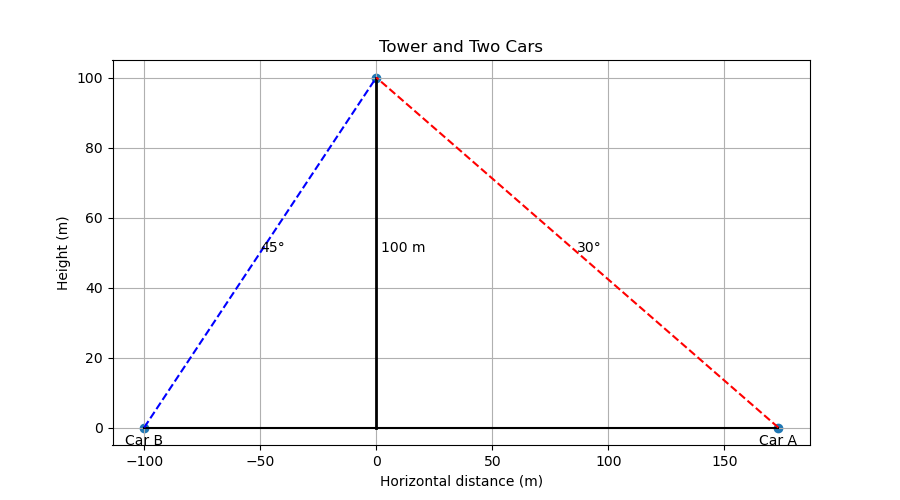
\includegraphics[width=0.75\linewidth]{figs/tower_cars.png}
    \caption{Tower and the two cars}
    \label{fig:EE26BTECH11229-8}
\end{figure}
\item 
In the given figure, O is the centre of the circle with $AC = 24$ cm, $AB = 7$ cm and $\angle BOD = 90^{\circ}$. Find the area of the shaded region.
\hfill (CBSE~2017)
\begin{figure}[H]
	\centering
\begin{tikzpicture}[scale=1.2]
\coordinate (O) at (0,0);
\coordinate (A) at (62.5:2.5);
\coordinate (B) at (30:2.5);
\coordinate (C) at (210:2.5);
\coordinate (D) at (-60:2.5);
% shaded regions: segment on AC, segment on AB, sector BOD
\fill[pattern=north west lines] (A) arc (62.5:210:2.5) -- cycle;
\fill[pattern=north west lines] (B) arc (30:62.5:2.5) -- cycle;
\fill[pattern=vertical lines] (O) -- (B) arc (30:-60:2.5) -- cycle;
% outlines
\draw (O) circle (2.5);
\draw (A) -- (C);
\draw (A) -- (B);
\draw (C) -- (B);
\draw (O) -- (D);
% right angle mark at O
\draw (30:0.25) -- ++(-60:0.25) -- (-60:0.25);
\fill (O) circle (0.04);
% labels
\node[above] at (A) {$A$};
\node[right] at (B) {$B$};
\node[left] at (C) {$C$};
\node[below] at (D) {$D$};
\node[above left] at (O) {$O$};
\end{tikzpicture}
\caption{}
    \label{fig:EE26BTECH11229-4}
\end{figure}
\solution
In \figref{fig:EE26BTECH11229-4}, $B$, $O$ and $C$ are collinear, so $BC$ is a diameter. From \eqref{eq:EE26BTECH11229-thales},
\begin{align}
	\angle BAC = 90^{\circ}, \quad BC = \sqrt{7^2 + 24^2} = 25 \text{ cm}
\end{align}
The radius is $r = \frac{25}{2}$ cm. Since $OD \perp BC$, $\angle COD = 90^{\circ}$ as well. The circle consists of the triangle $ABC$, the two segments on $AB$ and $AC$, and the two quadrants $BOD$ and $COD$. The shaded region is the two segments and the quadrant $BOD$, so its area is
\begin{align}
	A &= \pi r^2 - \text{ar}\brak{\triangle ABC} - \text{ar}\brak{\text{sector } COD}
	\\
	&= \pi r^2 - \frac{1}{2}\brak{7}\brak{24} - \frac{1}{4}\pi r^2
	= \frac{3}{4}\pi r^2 - 84
\end{align}
Substituting $\pi = \frac{22}{7}$ and $r^2 = \frac{625}{4}$,
\begin{align}
	A = \frac{3}{4}\times\frac{22}{7}\times\frac{625}{4} - 84
	= \frac{20625}{56} - 84 = \frac{15921}{56} \approx 284.3 \text{ cm}^2
\end{align}
The following code generates \figref{fig:EE26BTECH11229-10}
\begin{lstlisting}[frame=single, basicstyle=\rmfamily, escapeinside={(*@}{@*)}]
(*@\makebox[\dimexpr\linewidth-2\fboxsep-2\fboxrule\relax][c]{codes/shaded\_circle.py}@*)
\end{lstlisting}
\begin{figure}[H]
    \centering
    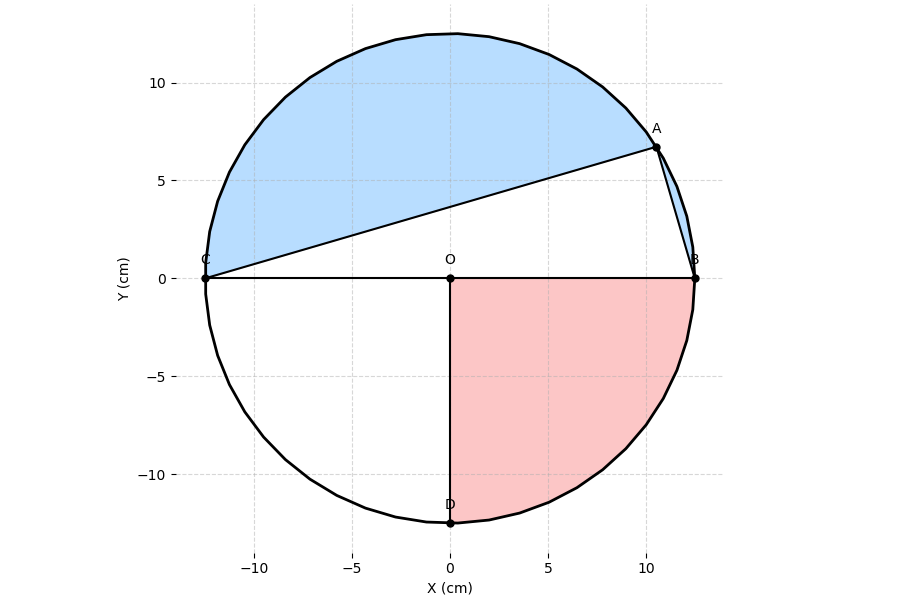
\includegraphics[width=0.75\linewidth]{figs/shaded_circle.png}
    \caption{Shaded region of the circle}
    \label{fig:EE26BTECH11229-10}
\end{figure}
\end{enumerate}
